Consider a circular plate under a uniform transverse load of $\bar q = 1.28\times 10^6$, the boundary of the plate is simply supported.
The material parameters of this plate is that $\bar D = 2\times 10^4$, $\nu = 0.3$.
The radius of the plate is $R=5$.
The plate occupies the full circular domain
\begin{equation}\label{circle_domain}
	\Omega = \left\{ \left(x,y\right) \mid x^2+y^2\le R^2 \right\}
\end{equation}
whose boundary is the circle
\begin{equation}\label{circle_outer_edge}
	\Gamma = \left\{ \left(x,y\right) \mid x^2+y^2=R^2 \right\}
\end{equation}
The simply supported condition is imposed on $\Gamma$ as
\begin{equation}\label{circle_outer_bc}
	w = 0, \quad M_n(w) = 0 \quad \textrm{on}\;\Gamma
\end{equation}
The corresponding meshfree discretization of the circular plate is shown in Fig. \ref{fig:circle_mesh}.

\begin{figure}[pos=htbp]
\centering
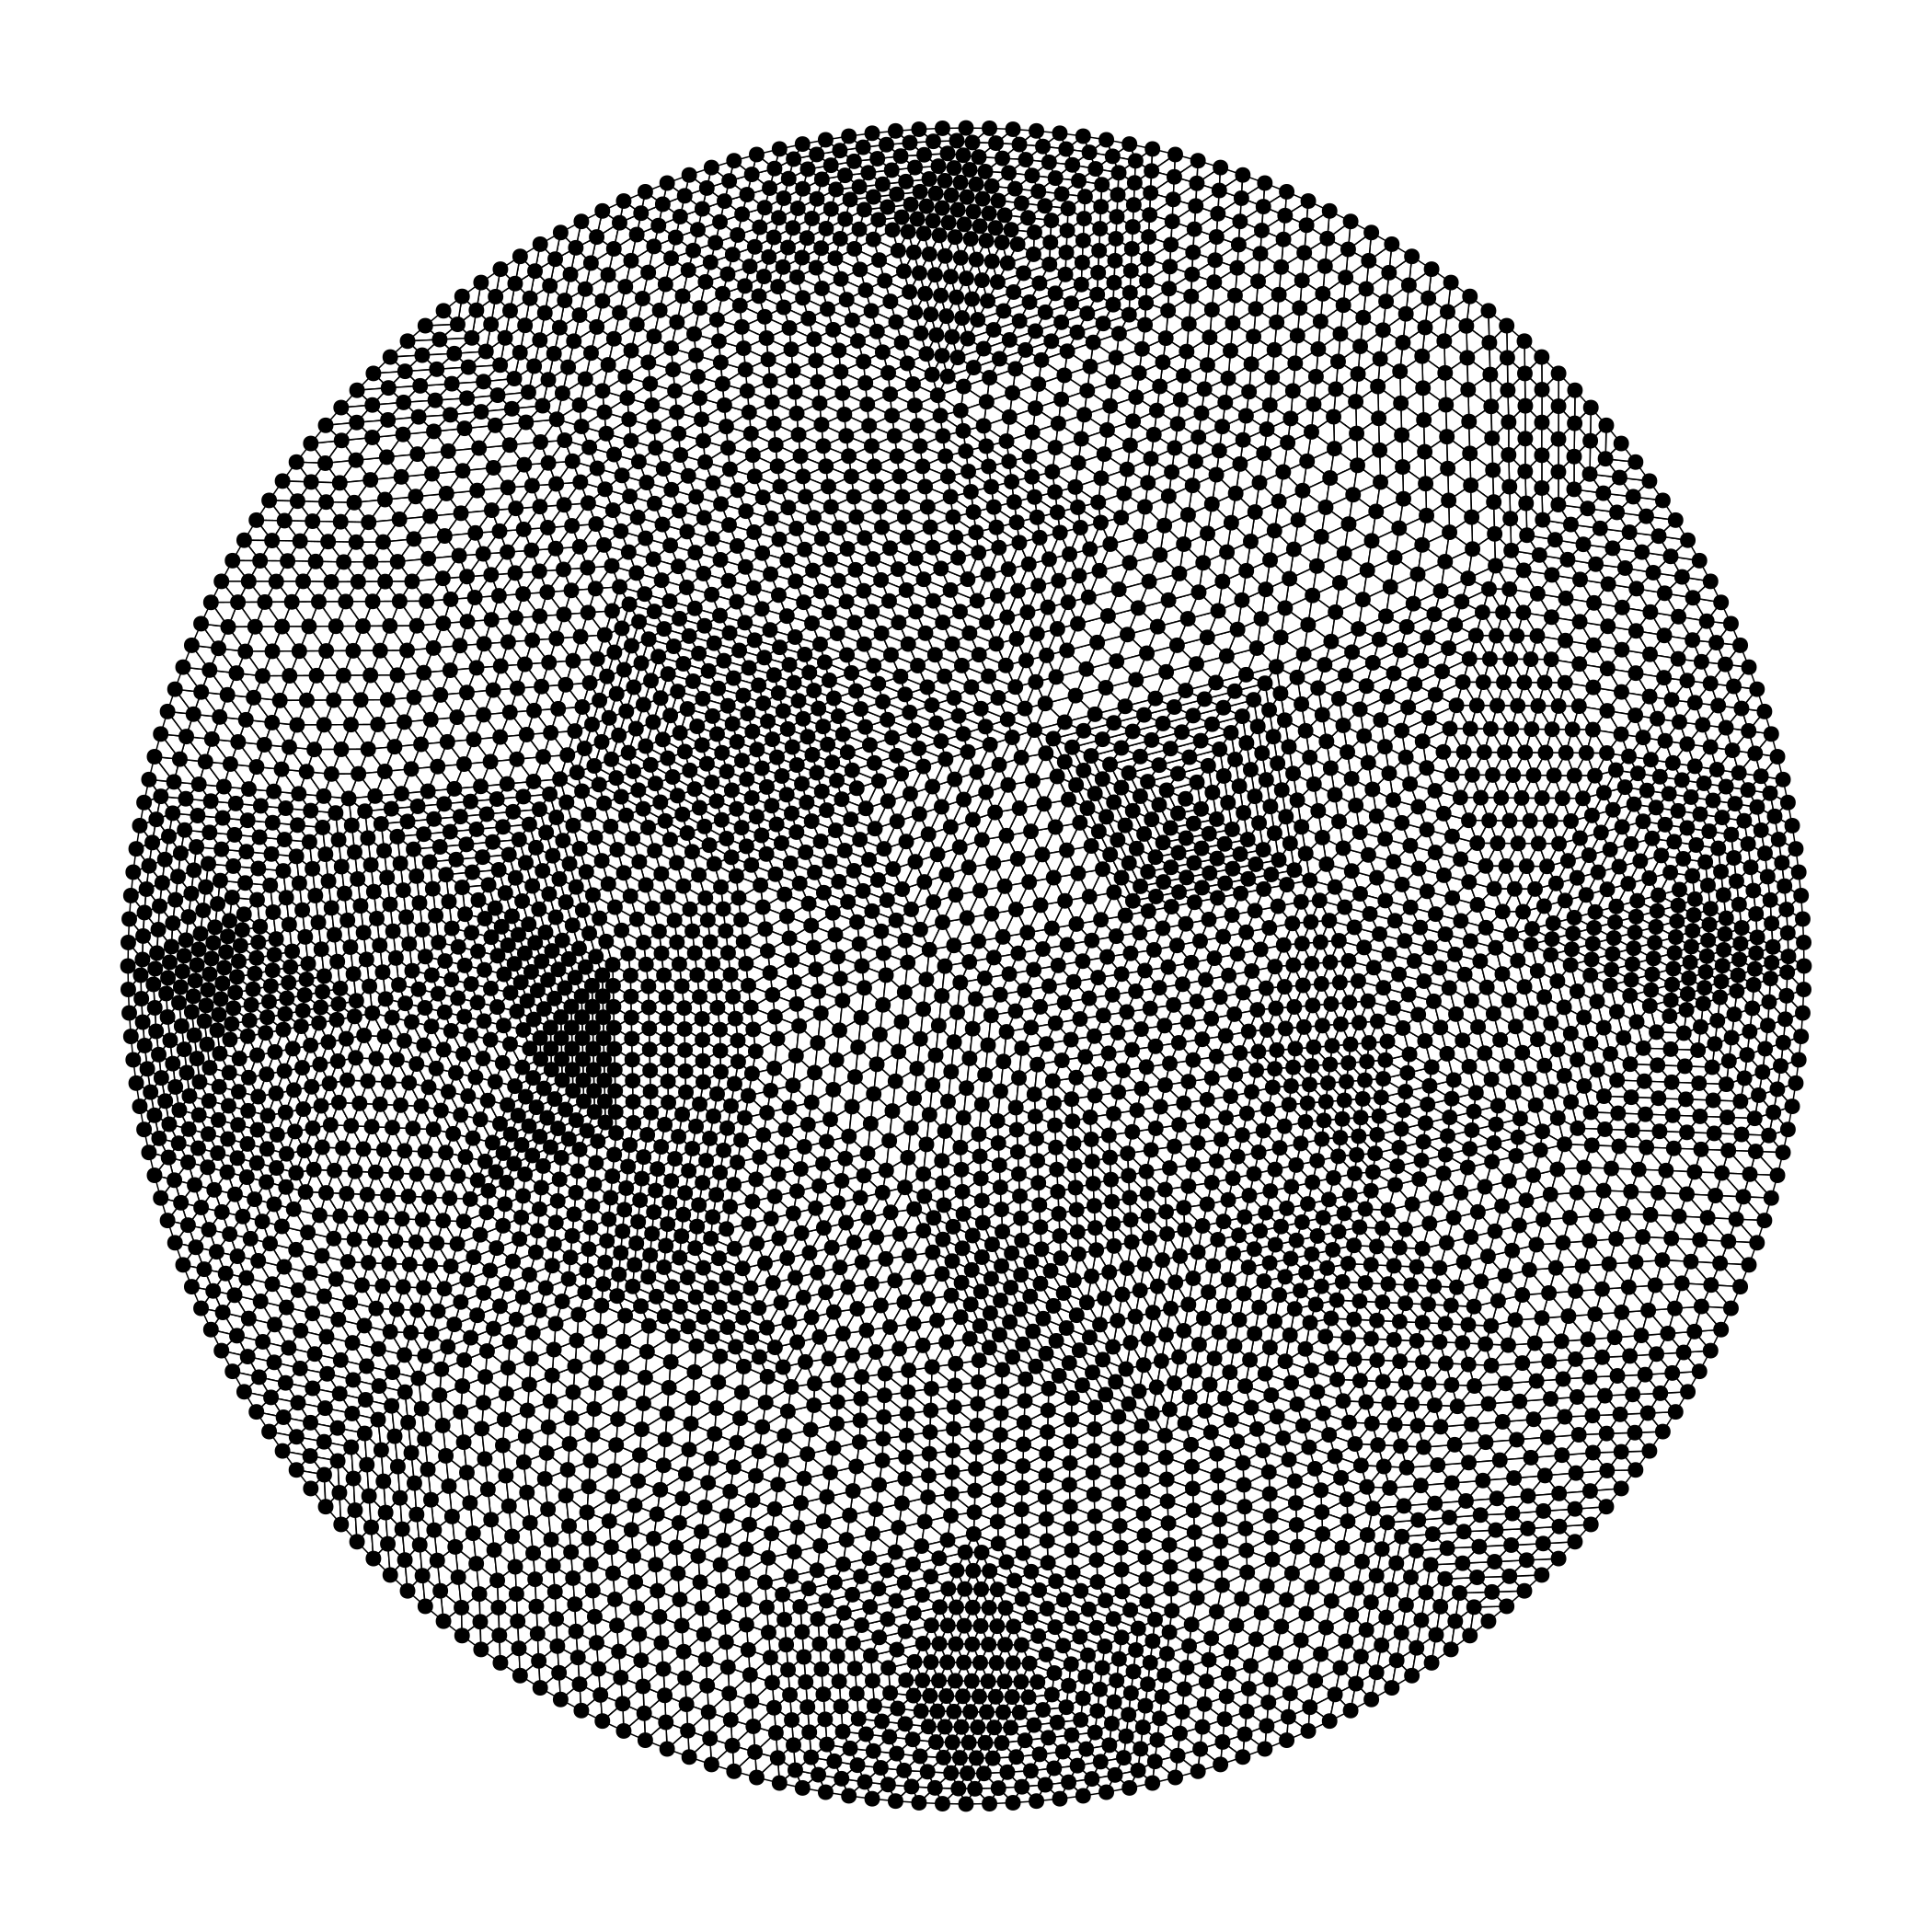
\includegraphics[width=0.45\textwidth]{figs/circle_mesh.png}
\caption{Meshfree discretization of the circular plate.}\label{fig:circle_mesh}
\end{figure}

The analytical solution of this problem states:
\begin{equation}\label{circle_exact}
	w = \frac{\bar q(R^2-r^2)}{64\bar D} \left( \frac{5+\nu}{1+\nu} R^2 - r^2\right)
\end{equation}
where $r = \sqrt{x^2+y^2}$ is the polar coordinate.
It can be verified that Eq. \eqref{circle_exact} satisfies the plate equation $\bar D w_{,iijj} = \bar q$ in $\Omega$, together with the simply supported boundary condition \eqref{circle_outer_bc}.
Moreover, the normal rotation $\theta_n(w)$ does not vanish on $\Gamma$, so Eq. \eqref{circle_exact} corresponds to the simply supported case rather than the clamped one.
